Let 
\begin{align}
\vec{A} = \myvec{-4 \\ 6 \\ 10} , \vec{B} = \myvec{2 \\ 4 \\6} , \vec{C} = \myvec{14 \\ 0 \\ -2}
\end{align}
Then 
\begin{align}
\vec{B-A}= \myvec{6\\-2\\-4},
\vec{C-A}=\myvec{18\\-6\\-12}
\end{align}
\begin{align}
\implies \vec{M} &= \vec{\myvec{B-A  & C-A}}^T
\\
 &= \myvec{6 & -2 & -4\\18 & -6 & -12} 
\xleftrightarrow {R_2 \rightarrow R_2-R_1}\myvec{6 & -2 & -4 \\12 & -4 & -8}
\end{align}
\begin{align}
\xleftrightarrow{R_2\rightarrow R_2-2R_1}\myvec{6 & -2 & -4 \\0 & 0 & 0}
\end{align}
\begin{align}
\implies \text{rank} \myvec{M} &=1
\end{align}
Thus, the points are collinear as can be seen in Fig. \ref{vec/2/27/fig: collinear}	
\begin{figure}[!ht]
\centering
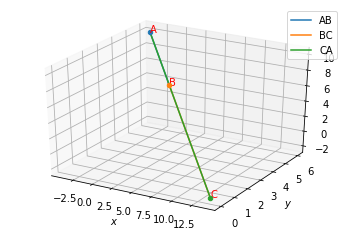
\includegraphics[width=\columnwidth]{solutions/su2021/2/27/Figure6.png}
\caption{collinear}
\label{vec/2/27/fig: collinear}	
\end{figure}
